\chapter{Experiments and Math Beauty}

\section{Experiment 1}
Is it possible to get a function that satisfies:
\begin{equation}
	\frac{d^n f}{dx^n}(n+1) = f^{(n)}(n+1) = 0 
\end{equation}

One of the possible answer (might be several) is 
\begin{eqnarray}
	f(x) &= \frac{1}{x^2} - \frac{1}{x} &= \frac{1}{x}\left(\frac{1}{x}-1\right)\\
	f'(x) &= \frac{-2}{x^3} + \frac{1}{x^2} &=-\frac{1}{x^2}\left(\frac{2}{x}-1\right)\\
	f''(x) &= \frac{3!}{x^4} - \frac{2!}{x^3} &=\frac{2}{x^3}\left(\frac{3}{x}-1\right)\\
	f'''(x) &= -\frac{4!}{x^5} + \frac{3!}{x^4} &=-\frac{3!}{x^4}\left(\frac{4}{x}-1\right)\\
	& \dots &\\
	f^{(n)} &= (-1)^n\frac{(n+1)!}{x^{n+2}}+(-1)^{(n+1)}\frac{n!}{x^{n+1}} &= (-1)^n\frac{n!}{x^{n+1}}\left(\frac{n+1}{x}-1\right)
\end{eqnarray}

for this we have
\begin{eqnarray}
	f^{(n)}(n) &=& (-1)^n\frac{(n-1)!}{n^{n+1}}\\
	f^{(n)}(n+1) &=& 0\\
	f^{(n)}(n+1) &=& (-1)^{(n+1)}\frac{n!}{(n+2)^{(n+2)}}
\end{eqnarray}

\begin{figure}[htbp]
	\centering
		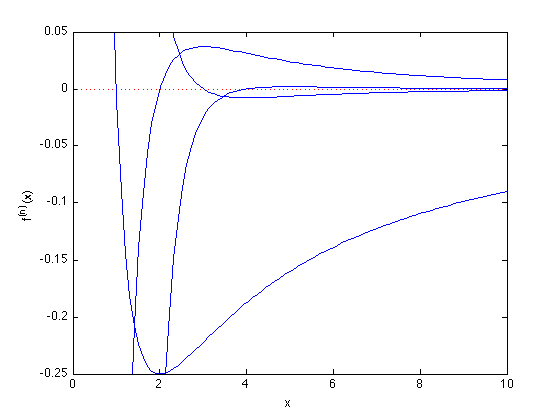
\includegraphics[height=4in]{images/crazyfunc.png}
	\caption{Illustration of $f^{(n)}(x)$ for $n=0, 1,2, 3$}
	\label{fig:images_crazyfunc}
\end{figure}
